%%%%%%%%%%%%%%%%%%%%%%%%%%%%%%%%%%%%%%%%%%%%%%%%%%%%%%%%%%%%%%%%%%
%%%%%%%% ICML 2016 EXAMPLE LATEX SUBMISSION FILE %%%%%%%%%%%%%%%%%
%%%%%%%%%%%%%%%%%%%%%%%%%%%%%%%%%%%%%%%%%%%%%%%%%%%%%%%%%%%%%%%%%%

% Use the following line _only_ if you're still using LaTeX 2.09.
%\documentstyle[icml2016,epsf,natbib]{article}
% If you rely on Latex2e packages, like most moden people use this:
\documentclass{article}

% use Times
\usepackage{times}
% For figures
\usepackage{graphicx} % more modern
%\usepackage{epsfig} % less modern

% For citations
\usepackage{natbib}

% For algorithms
\usepackage{algorithm}
\usepackage{algorithmic}

% As of 2011, we use the hyperref package to produce hyperlinks in the
% resulting PDF.  If this breaks your system, please commend out the
% following usepackage line and replace \usepackage{icml2016} with
% \usepackage[nohyperref]{icml2016} above.
\usepackage{hyperref}

% Packages hyperref and algorithmic misbehave sometimes.  We can fix
% this with the following command.
\newcommand{\theHalgorithm}{\arabic{algorithm}}

% Employ the following version of the ``usepackage'' statement for
% submitting the draft version of the paper for review.  This will set
% the note in the first column to ``Under review.  Do not distribute.''
\usepackage{icml2016} 

% Employ this version of the ``usepackage'' statement after the paper has
% been accepted, when creating the final version.  This will set the
% note in the first column to ``Proceedings of the...''
%\usepackage[accepted]{icml2016}


% The \icmltitle you define below is probably too long as a header.
% Therefore, a short form for the running title is supplied here:
\icmltitlerunning{Acoustic Fall Detection with Bagging Classifier}

\begin{document} 

\twocolumn[
\icmltitle{Acoustic Fall Detection using \\ 
           Bootstrap Aggregating (Bagging) Classifier }

% It is OKAY to include author information, even for blind
% submissions: the style file will automatically remove it for you
% unless you've provided the [accepted] option to the icml2016
% package.
\icmlauthor{Loukas Kominis}{loukaskom@gmail.com}
\icmladdress{University of Patras, Department of ECE, University campus Rio, Patras, Greece}
\icmlauthor{Your CoAuthor's Name}{email@coauthordomain.edu}
\icmladdress{Their Fantastic Institute,
            27182 Exp St., Toronto, ON M6H 2T1 CANADA}

% You may provide any keywords that you 
% find helpful for describing your paper; these are used to populate 
% the "keywords" metadata in the PDF but will not be shown in the document
\icmlkeywords{acoustic,bagging,svm,knn,machine learning}

\vskip 0.3in
]

\begin{abstract} 
A different approach on designing an Acoustic Fall Detection system, is presented. This kind of system is ideal for different smart environments, like an office, home etc. which embed just simple microphones. Better scores in all categories were accomplished, with the implementation of a new classifying method, different from what previous researches on this field propose.
\end{abstract} 

\section{Introduction}
\label{introduction}

Nowadays, smart homes and smart environments are significantly increasing with a lot of connected devices in them. As engineers, it is important to benefit from their presence and use them to solve human needs. Falls are a public health problem, especially in environments with elder and disabled people. In smart homes today it is really challenging to manage helping people with such needs. 

Worldwide statistics  show that 28-35\% of people aged of 65 and over fall every year with this percentage increasing to 32-42\% for people over 70 years old. Furthermore, the research indicates that around 30\% of falls lead to injuries that require medical assistance for several days and account 40\% of all injury deaths. It is clear, that assistance in this area can be really helpful and in some cases crucial for a person's health.

But providing assistance in this cases through modern technology is a challenge that has multiple difficulties to face. First, it is just the technical level, where we need to overcome all possible obstacles and be innovative in order to use technology in the best possible way to help people. Second, there is also a social level. And this is really important for people. It is a fact, that technology is present to most of our everyday activities year by year passing. This higher accessibility though can also have disadvantages. Today, we can refer to technology and describe it as “intrusive” - “non-intrusive”, “confidential” or “non-confidential”. It's on our hands as engineers to decide which of these describe our systems or products and make people to trust our work and assistance. 

This is the vision of Qarnot Computing, to provide through its products assistance and trust-worthy services to its clients. Qarnot computing [1] promotes a cloud computing model where heating, computing, storage and networking is provided from a single infrastructure: a network of geo-distributed servers deployed in homes, offices and buildings. The Qarnot model is based on two main products. The first is a new model of servers (Q.rads) in which the cooling system is replaced by a heat diffusion system, regulated by a thermostat. Each Q.rad (See Figure 1) embeds several processors in addition to sensors related to humidity, CO 2 , presence etc. The second Qarnot product is a new middle-ware (Q.ware) for on-demand computing. Q.ware manages two types of requests: requests for processing cloud services and requests for heating. Its goal is to deploy and adjust the run of cloud workloads to meet the heat demand on Q.rads. For more details about the Qarnot model, we refer the interested reader to [2].

So having Q.rads, which also embed microphones, we visioned on create a system to make the smart home safer and more assistive to people. As among their other functions, Q.rads are also heaters, this means that they can be present to most places in a closed environment such as a house. So the smart home containing now Q.rads can be much safer with an Acoustic Fall Detection system. 

Our vision is to have an independent system that can identify a fall just from audio data and with further improvement in the future possibly alert the public health services or some relatives. Or as a second option be supportive to a general fall detection system and improve its accuracy by a good percentage that can reach 5-10\%. 

In the majority of previous researches on this field, people mostly used accelerometers or cameras to create similar systems. But our opinion is different and we believe that a system like this can be accomplished just with audio data and still be successful. In this experimental research what we present is that with the use of a new classification method, from the ones used in previous researches, we can accomplish better scores and higher accuracy. Bootstrap Aggregating (Bagging) is used to classify falls, after having trained SVM and KNN classifiers in order to provide results of the better scores that can be achieved with Bagging to such a case of zero-one classification problem.

\begin{figure}[t]
\begin{center}
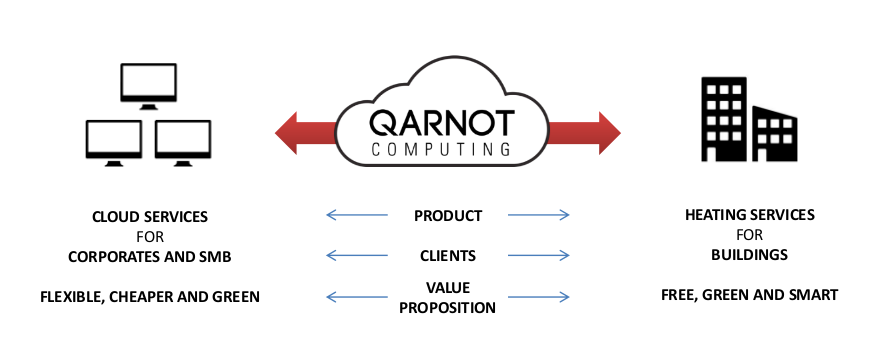
\includegraphics[width=10.7cm,height=3.5cm]{./Figures/model.png}
\caption{\scriptsize The roles of the Q.ware }
\end{center}
\end{figure} 

So this paper is organized in different sections to show the whole procedure. In section 1, it is described how our dataset used to train different classifiers was created. Section 2, refers to the training of SVM and KNN classifiers and the results they produced. In section 3, Bagging classifier is trained with different parameters and results are shown to prove our theory. Section 4, is conclusion and discussion about further improvement of this system.

\section{Creating the Dataset} 
 
In order to be able to design an accurate system, it is really important to create a good dataset. As for a system like this, it is not easy to create a dataset from zero, we used as main source an already existing Laboratory research dataset [3]. It contained video data which consisted of falls and other no-fall activities in different environments and especially Office, Home, Coffee room and Lecture room. The frame rate is 25 frames/s and the resolution 320x240 pixels. The dataset containes 191 videos of different time durations, from 6 sec to 1.20 minutes. The use of different environments makes the dataset more complete and representative in compare to others.  

\subsection{Audio Extraction}

Using the Audacity software, we extracted the audio and isolated the fall and no-fall segments. The duration of the segments is 5 seconds. Also a re-sampling was done to the audio files in order to have the same sampling rate (44100 Hz) in all of them and they were also converted to monophonic so that they can be used by our python code and libraries used.

\subsection{Noise Mixing and Features extraction}

Next step of the procedure was the audio files to get mixed with different types of noise (in all available combinations), so that our dataset is an accurate representation of real-life everyday sounds. At the end, the dataset consists of two major categories, Falls and No-falls, each of them containing a big variety of samples from all the different environments that were used to record the videos. So it is clear that our dataset in now complete. After finishing with the creation of the dataset, next step is to extract the features needed to run the algorithms. For this purpose, an open source library was used, the pyAudioAnalysis python library [4] which extracts specific features for each audio file. These features will be used to train the machine learning algorithms.

\subsection{Subsets creation}

The last step to the dataset creation, is to split it in Training and Testing subsets. The proportion remains constant for the entire duration of this experimental research project. Training subset includes 80\% of the main dataset samples and Testing subset 20\%. This split is required in order to produce learning curves for each classifier and also have cross-validation during training them.

\section{SVM and kNN implementation}

In this Section, SVM and kNN classifiers are trained on the dataset previously created. In this Section we present the work done in four experimentation Phases, where the algorithms run in different proportions of data and cover all possible scenarios. The proportion of falls and no falls will be increased and decreased respectively in each Phase in order to check how the algorithms respond on the amount of data given.

The Scikit-Learn python library is used for importing the code, needed for the classifiers, to our main python code. Scikit-Learn library was selected as it provides an easy, universal way for importing different classifiers. 

In each classifier used, after training is finished, which is done using the Q.ware platform and actual Q.rads, the five most efficient classifiers are selected and a choice of the best one is made, among them, based on shortest training time. The most important part is the evaluation of the classifier, where the best classifier is used on both Testing and Training Dataset and see through the Learning Curves and the scores of the confusion matrix, which are presented, how the classifier responds as the amount of data is increasing. 

\subsection{Phases workflow and results}

In total this section consists of four Phases. In each of them, a different proportion of fall and no fall data was used in order to check the response of the algorithms. In Table 1, the proportions and total amount of data are presented for each Phase. 

In Phase 1, only SVM classifier is trained and we chose to begin with this specific one as it is mostly used to other researches. The results though were definitely not what we expected as at first True-positive rate is really low and False-positive rate seemed unrealistic as a value. The duration of audio data in this phase (audio segment of fall or no fall mixed with noise) was 10 seconds and proportion of falls and no falls was 20-80\%. 

In Phase 2, it was decided to reduce duration of the audio data to 5 seconds in order to make it easier for the classifier to detect the fall part. It will also make the training faster. Falls and no falls proportion was 40-60\%. Also the KNN classifier was introduced and trained for the first try as an effort to compare results with SVM. Better results were produced to the SVM, as the True-positive rate increased by 20\%. KNN had similar scores to the SVM as shown in the table, but in general these results are not yet acceptable in order for our system to be independent. 

So moving on to Phase 3, SVM and KNN classifiers were trained again, duration of audio data is still 5 seconds and proportion of data is changed to 50-50\% and we hoped to improve more the scores of the classifiers. But, the SVM results were dissapointing. Instead of improve, they deteriorated. KNN on the other hand, had better results. This difference in the results can be explained by the different definition of the two classifiers. As KNN detects similarities in a close nearby area it is profited by adding more fall data. In this phase, it was when we first thought of having a different approach on the way of classification, as the system seems to have a kind of sensitivity to the amount of data given each time, that it is not easy to regulate. 

As it was needed to see if our thoughts had basis, we moved on to Phase 4. Here, the same settings are used, except the proportion of data used, which changed to 60-40\% of falls and no falls. And the results, certified our theory of sensitivity. The SVM classifier, had a significant improvement and for sure these were the best scores achieved with this specific classifier. KNN still produced good results but not with such a huge improvement to its scores. 

By checking the results shown in Table 2, which presents the scores of each classifier for all four experimentation Phases, the above described are more clear. Three are the categories presented. False-positive-rate (F.P.R), True-positive-rate and Accuracy.  

\begin{table}[ht]
\caption{Proportions of data, for each Phase}
\label{Data}
\begin{center}
\begin{small}
\begin{sc}
\begin{tabular}{lcccr}
\hline
\abovespace
Phase & Fall & Fall(\%) & No Fall & No Fall(\%) \\
      & Samples &        & Samples &            \\ 
\hline
\abovespace
1    & 1600 & 20 & 4800 & 80 \\
\hline
\abovespace
2    & 2400 & 40 & 4000 & 60 \\
\hline
\abovespace
3    & 3200 & 50 & 3200 & 50 \\
\hline
\abovespace
4    & 4000 & 60 & 2400 & 40 \\
\hline
\end{tabular}
\end{sc}
\end{small}
\end{center}
\vskip 0.1in
\end{table}

\begin{table}[t]
\caption{Classifiers scores, in each Phase}
\label{Scores}
\vskip 0.1in
\begin{center}
\begin{small}
\begin{sc}
\begin{tabular}{lcccr}
\hline
\abovespace
Phase & Classifier & F.P.R & T.P.R & Accuracy\\
\hline
\abovespace
Ph.1    & SVM & 0.00 & 0.18 & 0.79 \\
\hline
\abovespace
Ph.2    & SVM & 0.12 & 0.45 & 0.75 \\
     & KNN & 0.10 & 0.42 & 0.73 \\
\hline
\abovespace
Ph.3    & SVM & 0.40 & 0.20 & 0.40 \\
	 & KNN & 0.17 & 0.78 & 0.80 \\
\hline
\abovespace
Ph.4    & SVM & 0.20 & 0.92 & 0.90 \\
	 & KNN & 0.21 & 0.79 & 0.77 \\
\hline
\end{tabular}
\end{sc}
\end{small}
\end{center}
\vskip -0.3in
\end{table}

\subsection{Conclusion}

After testing SVM and KNN classifiers in different amount of data and comparing their scores, it is clear that this kind of system behaves differently depending on the amount of data given each time. The SVM results leave no doubt to this statement. KNN has better scores, but as explained previously it is due to the way it works and classifies falls. Our main accomplishment is the one presented on next section.
 
\section{Bootstrap Aggregating}

The results of the previous results, made us considering a different approach for this type of system. The data sensitivity issue had to be solved. So in this Section, a new classifier is introduced in order to help us achieve better scores and easier classification of falls and solve the data sensitivity issue. Bootstrap Aggregating, commonly known as Bagging, is an ensemble meta-estimator. It is important to give an explanation of Bagging in order to make clear for the reader, how we think it can help us. Bagging classifier establishes base estimators to randomly selected subsets of our main dataset. Then it aggregates their estimation to produce one final estimation for the entire dataset. This is its main advantage against other methods. 

The randomly selected subsets assure that we can have an estimation for all possible combinations of data instead of choosing a fixed proportion. Furthermore, the idea of base estimators, aggregated to a final estimation, gives the opportunity to combine all estimations, in an effort to consider parts of the dataset were classification is done properly and other where it is not. 
So this section is also split in Phases. But with some differencies from the previous one. Here proportion of data is kept stable for every Phase and is 50-50\% of falls and no falls, so that we can have enough samples of both categories. The duration of audio data is still 5 seconds. 
What is getting different at each Phase are the estimators, in an effort to see if we can achieve better results than the classifiers used in previous section. 

\subsection{Decision Tree base estimators}

The first approach of classification with Bagging method was done using it's default parameters which include Decision Tree base estimators. The results produced were more than satisfying. They were much better than our initial expectations. Except from the fact that False-positive rate is under 20\% combined this time with a True-positive rate which significantly increased to 90\%, also Accuracy reached 90\% and the Learning curves also represent a system with stable improvement as more data were given to it. 

\subsection{kNN base estimators} 

As the results of the previous Phase were really promising and much better than any previous try, it was decided make some simulations with other base estimators. In this phase, KNN base estimators were selected in an try to see if better results than the KNN classifier alone, can be produced. And as the results presented in Table 3, prove that this is a goal that can be achieved.  

\subsection{SVM base estimators}

After running Bagging Classifier with Decision Tree and kNN estimators it was also really important to try it with SVM estimators in a try to have also in this category better results in prove our theory of data sensitivity which we hope to solve via the Bootstrap Aggregating method. 

\begin{table}[hb]
\caption{Bagging Classifier scores with different estimators}
\vskip 0.1in
\begin{center}
\begin{small}
\begin{sc}
\begin{tabular}{lcccr}
\hline
\abovespace
Estimator & F.P.R & T.P.R & Accuracy\\
\hline
\abovespace
Decision Tree & 0.16 & 0.90 & 0.87 \\
\hline
\abovespace
KNN & 0.22 & 0.88 & 0.84 \\
\hline
\abovespace
SVM & 0.xx & 0.xx & 0.xx \\
\hline
\end{tabular}
\end{sc}
\end{small}
\end{center}
\vskip -0.2in
\end{table}

\subsection{Figures}

After presenting the scores for each classifier trained, what is also an important tool for machine learning are Learning curves. This section is dedicated to the Learning curves of the classifiers trained during the different phases of this project. 
It is important to see who the system can benefit from adding more data. 

\begin{figure}[h]
\vskip 0.2in
\begin{center}
\centerline{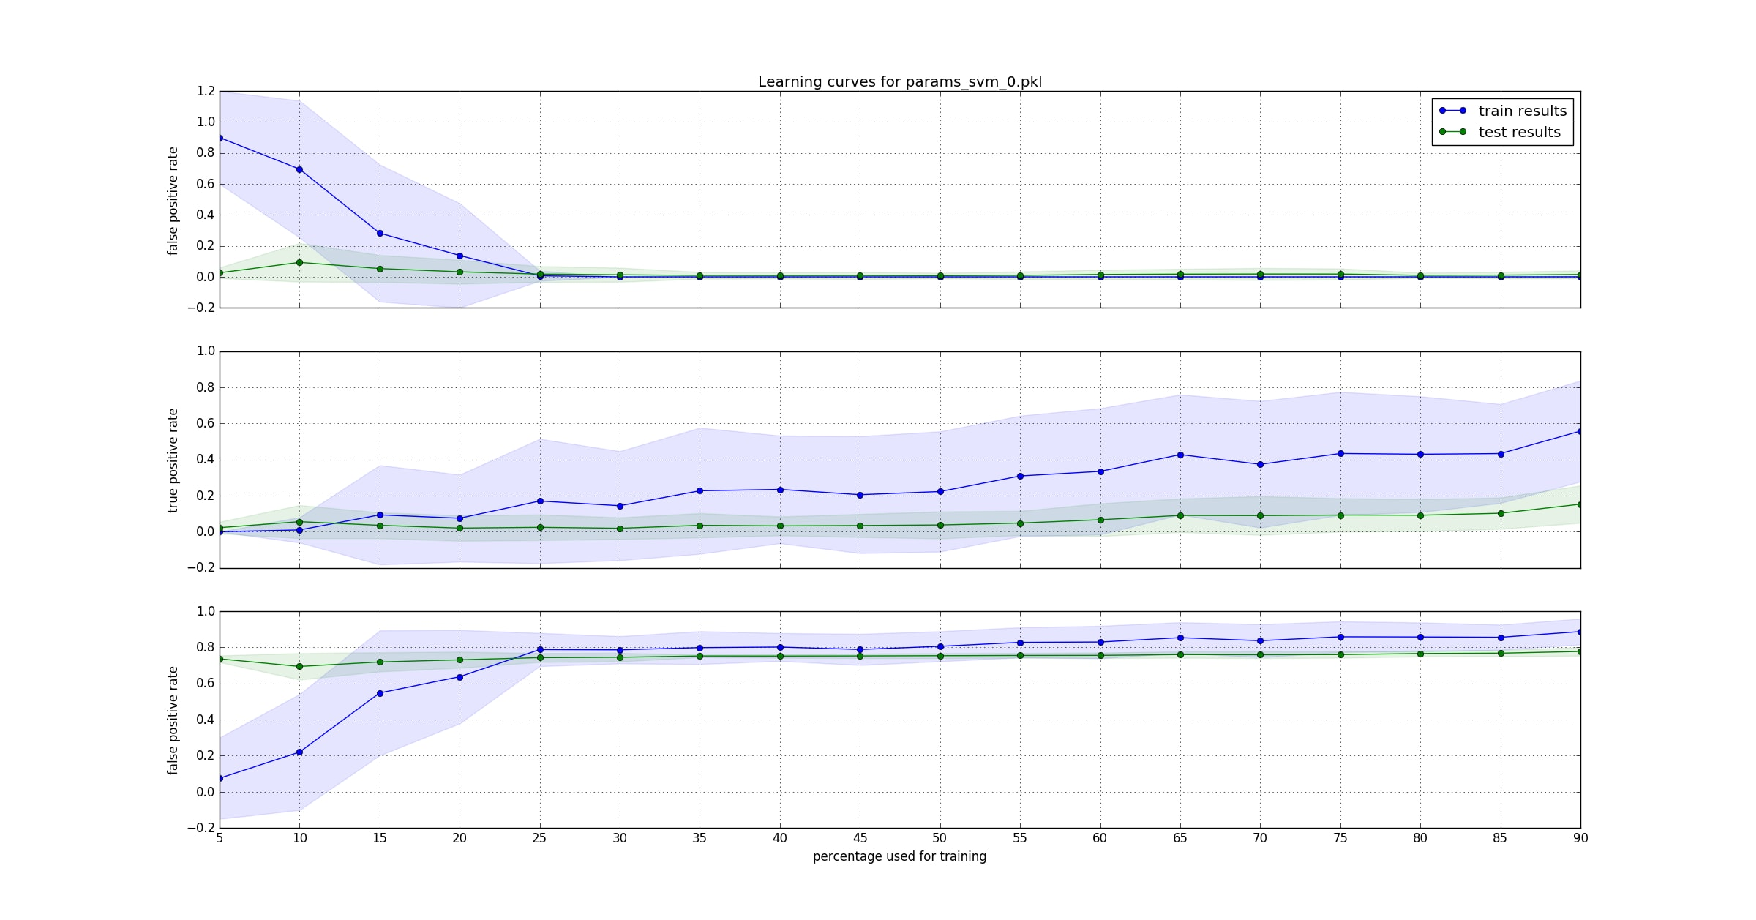
\includegraphics[width=\columnwidth, scale=1]{Lc_Ds1_P20-80_SVM}}
\caption{Learning curves, Phase 1, SVM}
\label{learning curves}
\end{center}
\vskip -0.2in
\end{figure} 

\begin{figure}[h]
\vskip 0.2in
\begin{center}
\centerline{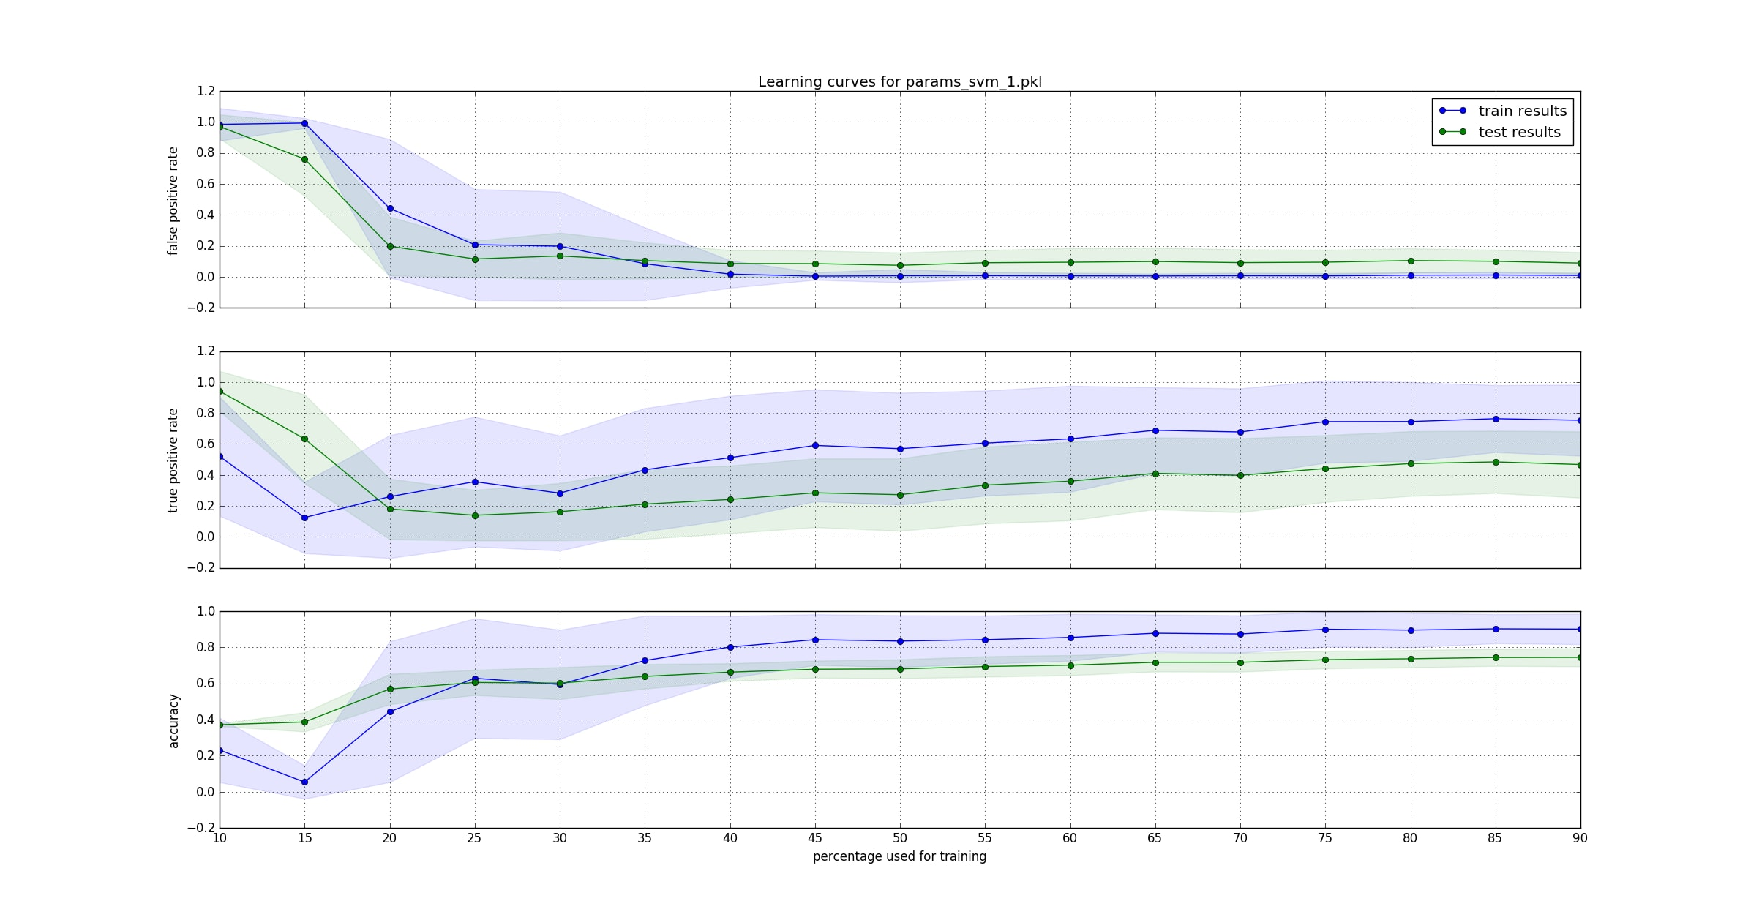
\includegraphics[width=\columnwidth, scale=1]{Lc_Ds2_P40-60_SVM}}
\centerline{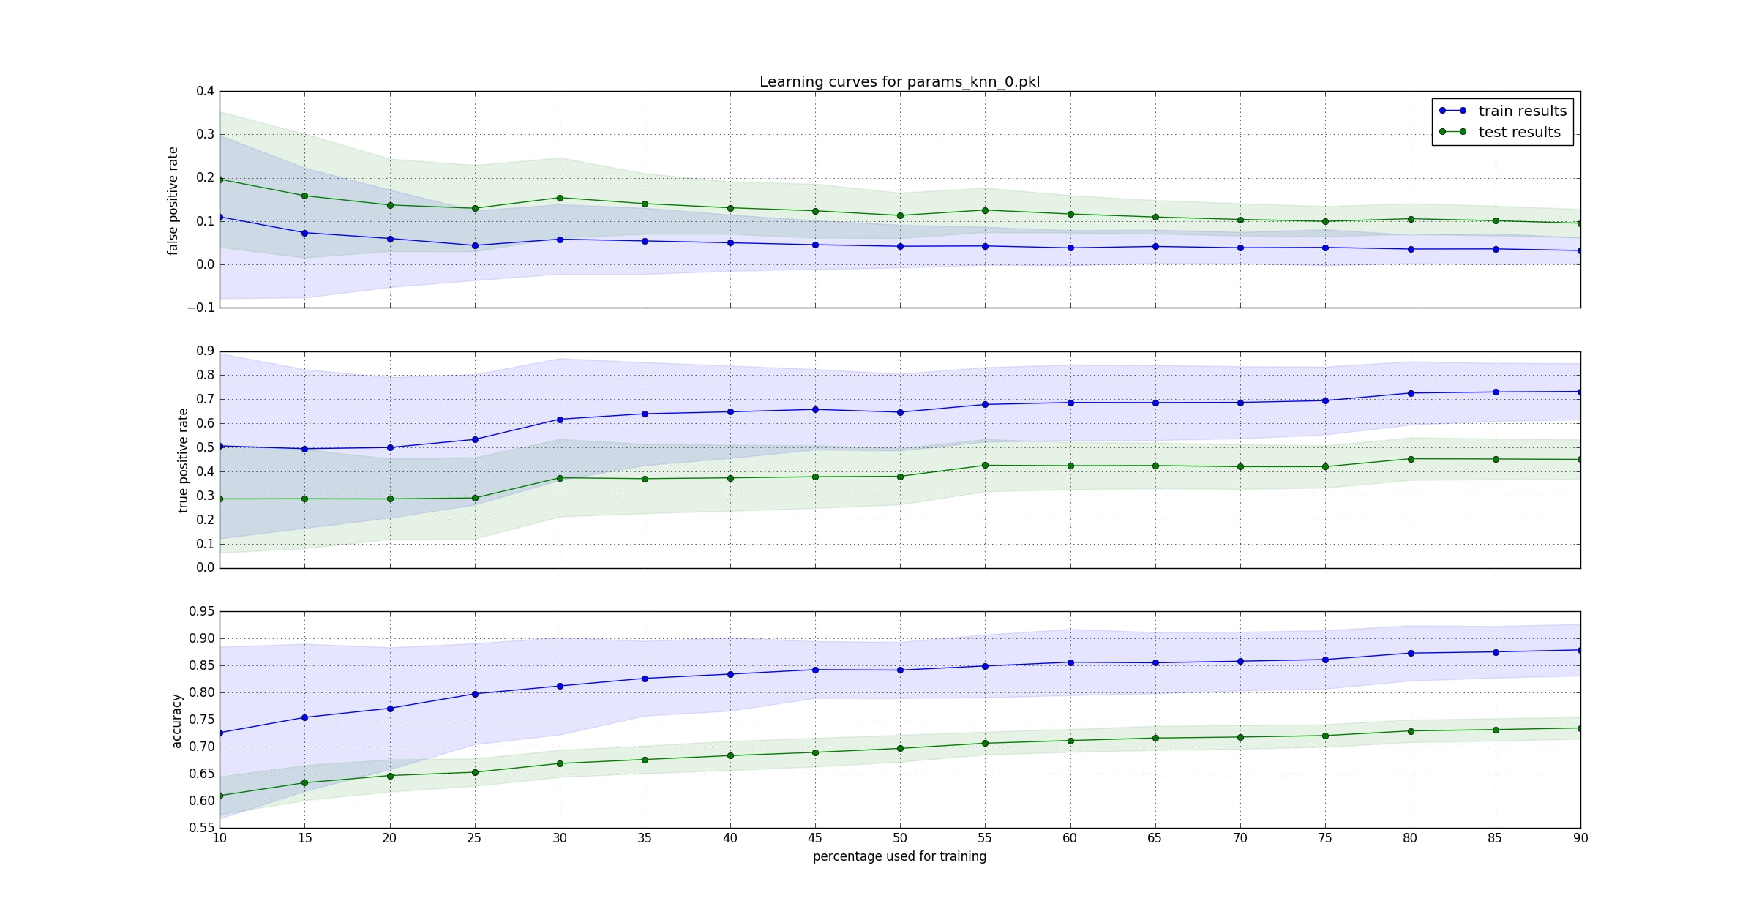
\includegraphics[width=\columnwidth, scale=1]{Lc_Ds2_P40-60_kNN}}
\caption{Learning curves, Phase 2, SVM& and KNN}
\label{learning curves}
\end{center}
\vskip -0.2in
\end{figure} 

\begin{figure}[h]
\vskip 0.2in
\begin{center}
\centerline{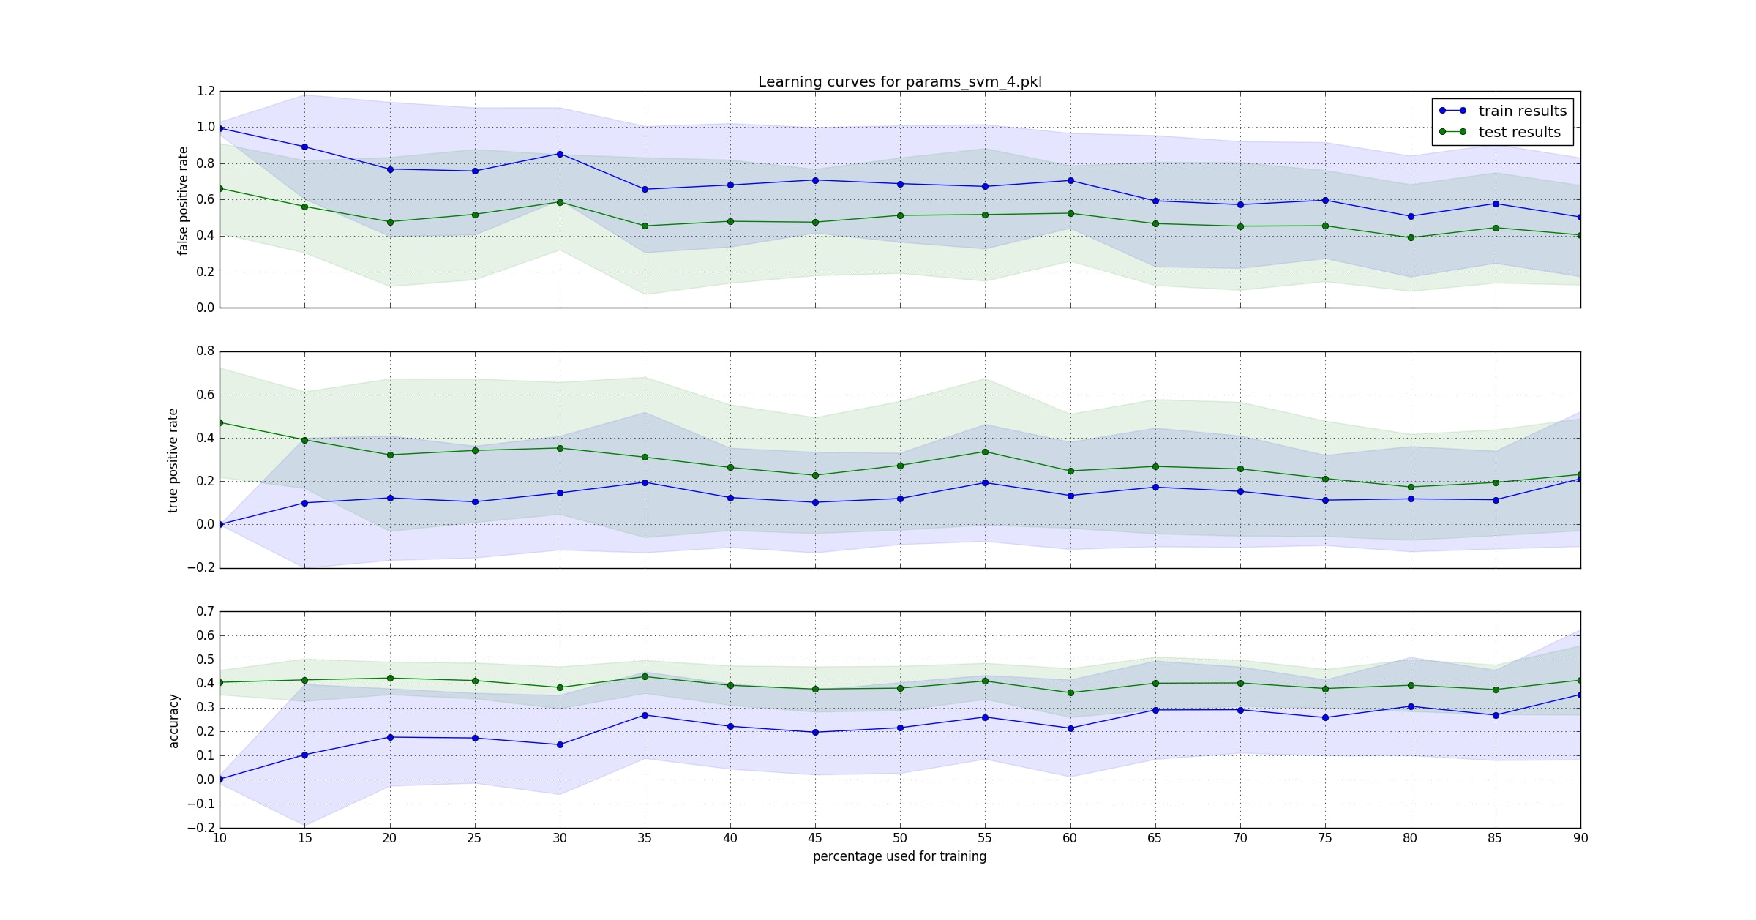
\includegraphics[width=\columnwidth, scale=1]{Lc_Ds3_P50-50_SVM}}
\centerline{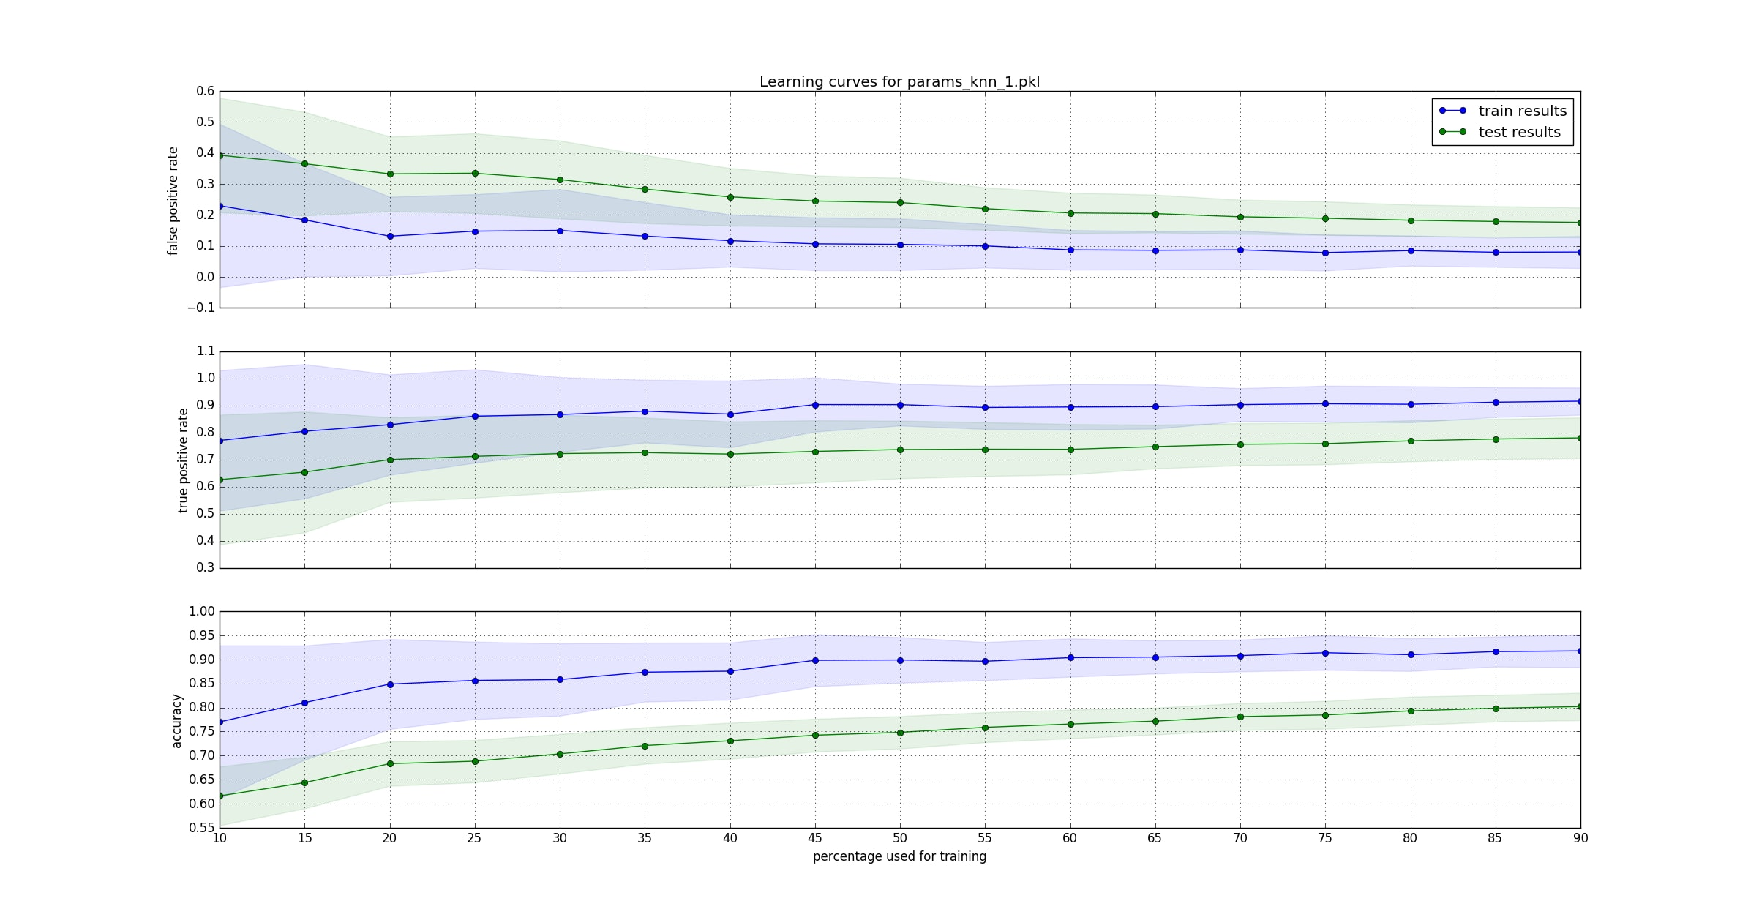
\includegraphics[width=\columnwidth, scale=1]{Lc_Ds3_P50-50_kNN}}
\caption{Learning curves, Phase 3, SVM and KNN}
\label{learning curves}
\end{center}
\vskip -0.2in
\end{figure} 

\begin{figure}[h]
\vskip 0.2in
\begin{center}
\centerline{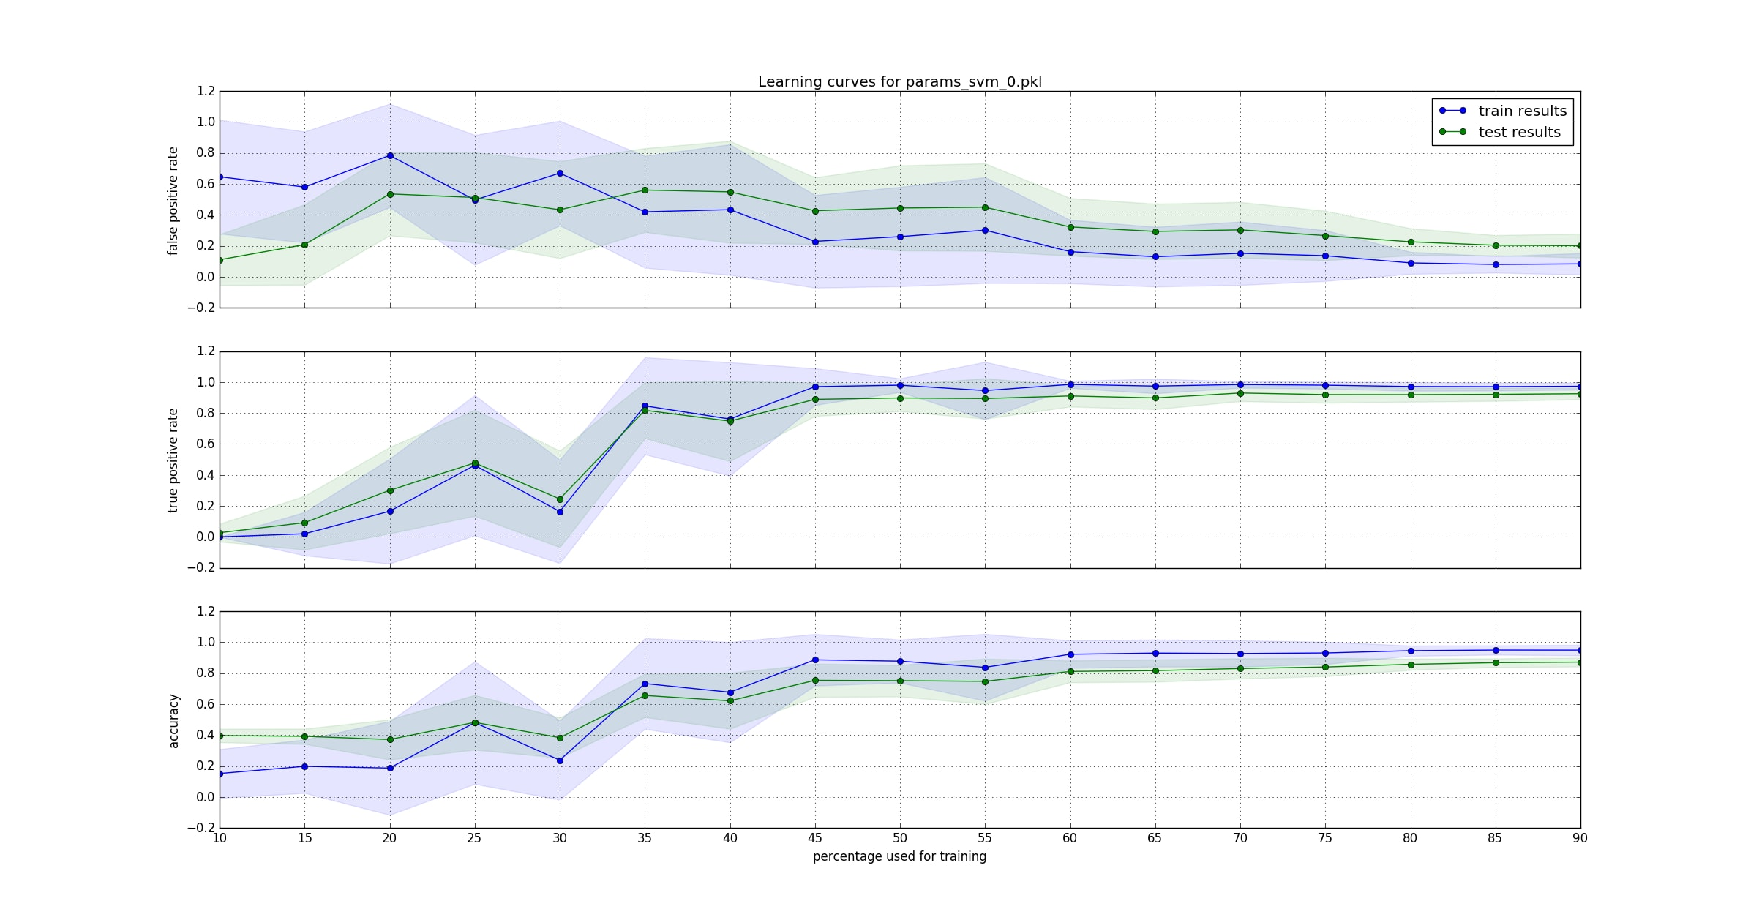
\includegraphics[width=\columnwidth, scale=1]{Lc_Ds4_P60-40_SVM}}
\centerline{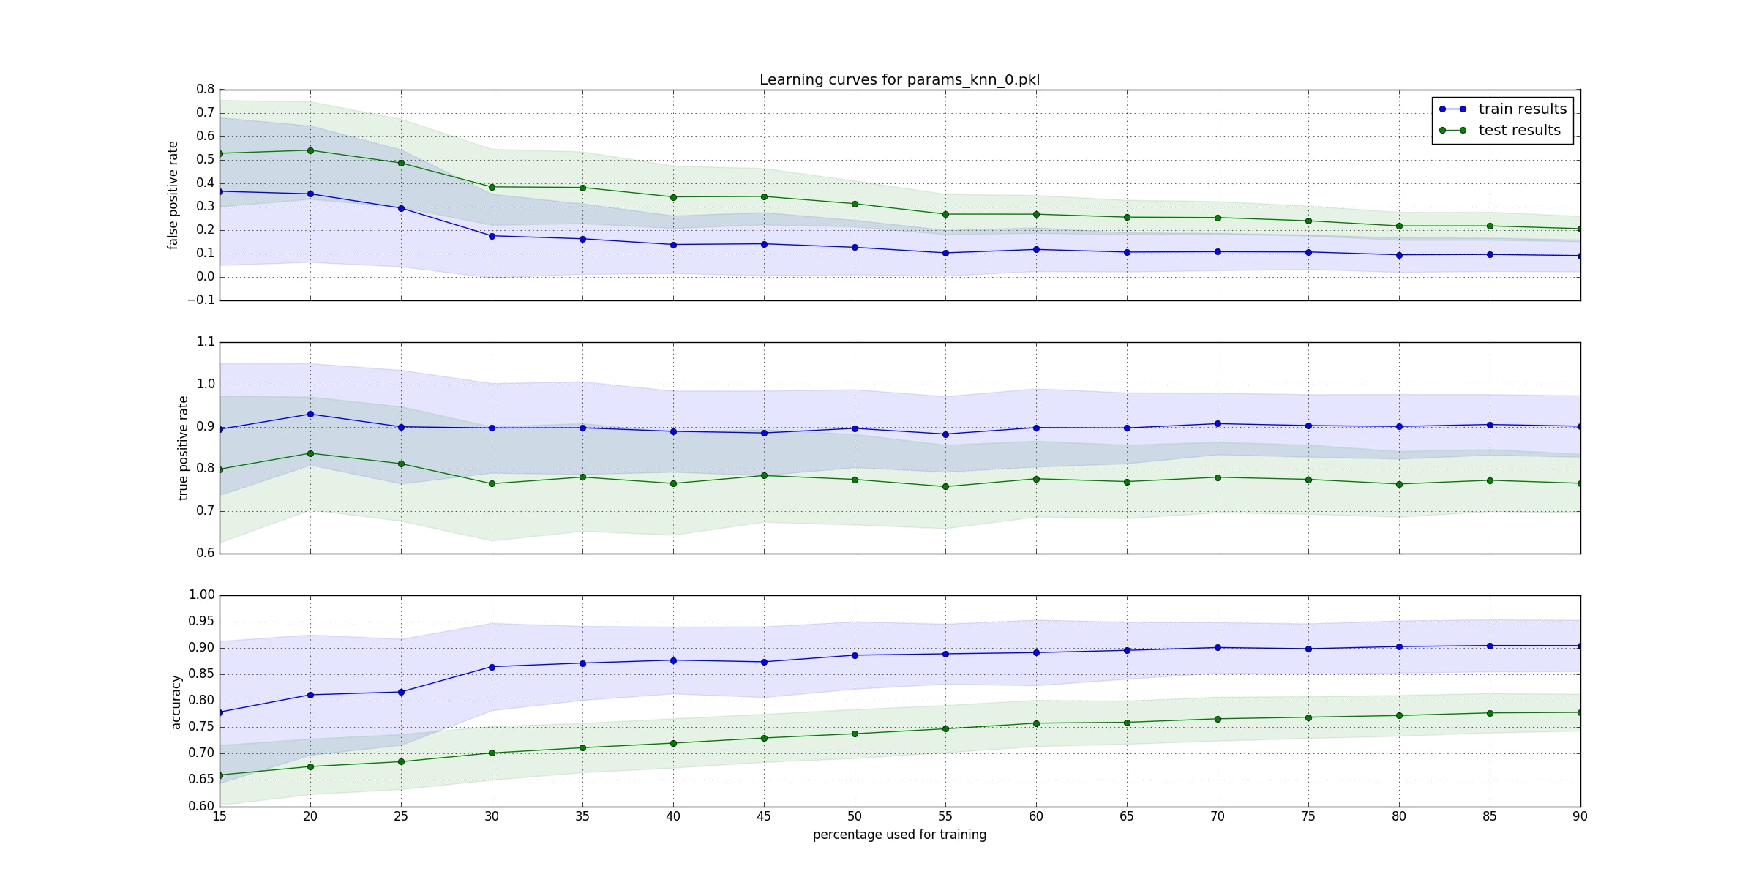
\includegraphics[width=\columnwidth, scale=1]{Lc_Ds4_P60-40_kNN}}
\caption{Learning curves, Phase 4, SVM and KNN}
\label{learning curves}
\end{center}
\vskip -0.2in
\end{figure} 

\begin{figure}[h]
\vskip 0.2in
\begin{center}
\centerline{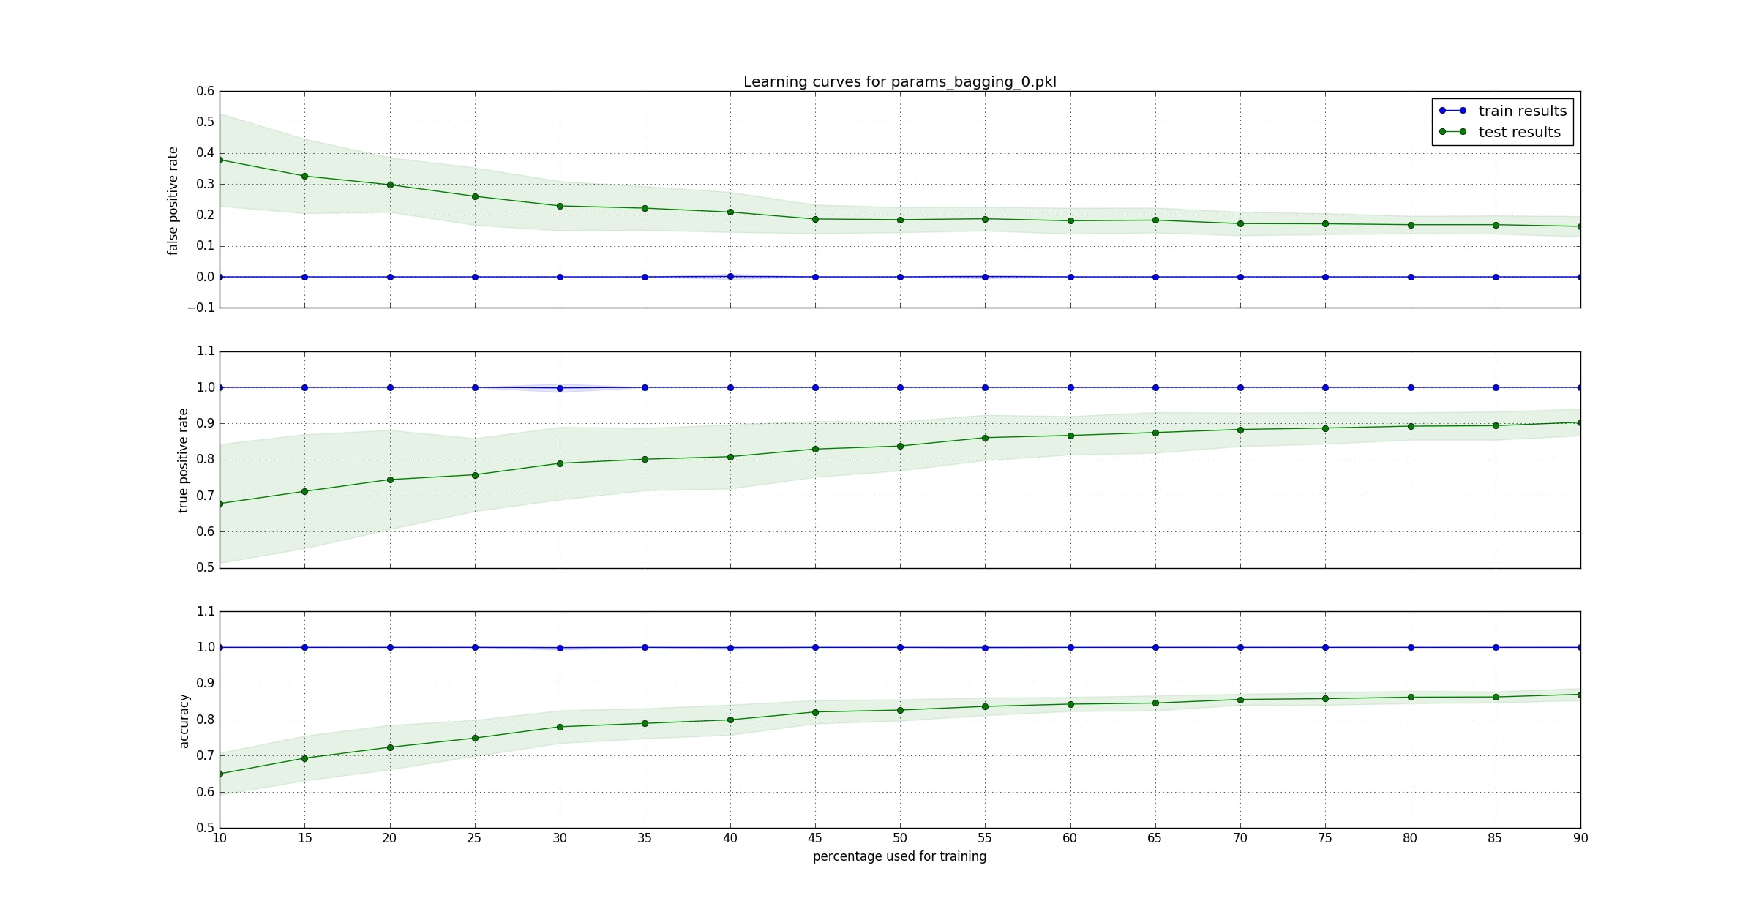
\includegraphics[width=\columnwidth, scale=1]{Lc_Ds5_P50-50_BaD}}
\centerline{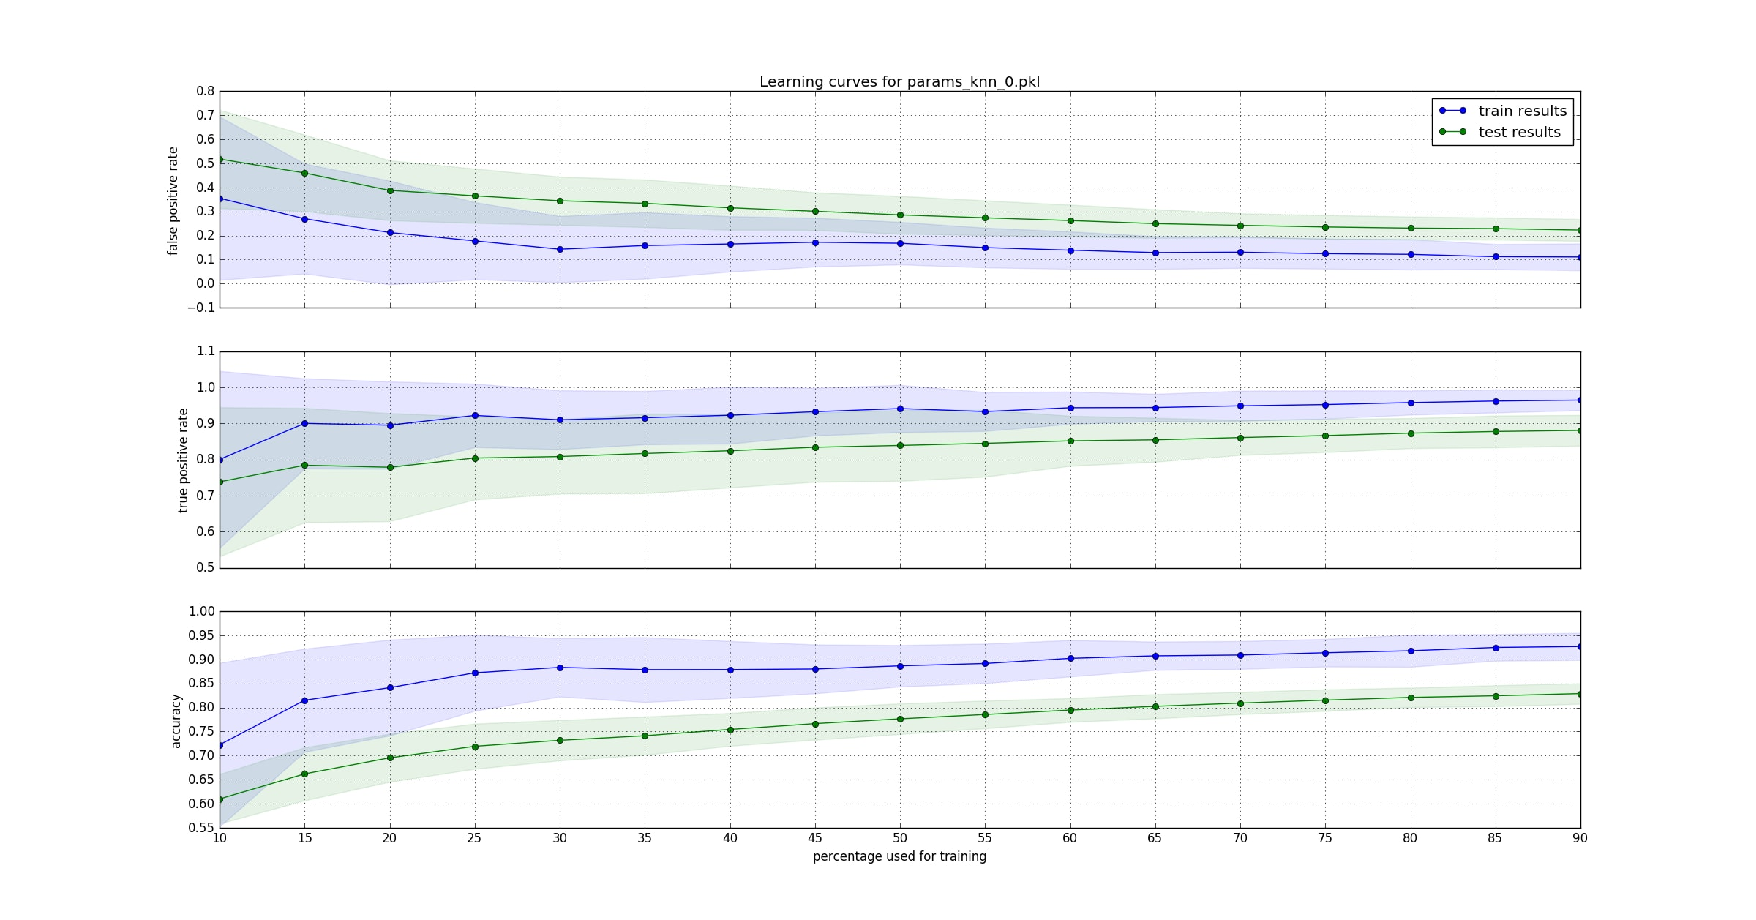
\includegraphics[width=\columnwidth, scale=1]{Lc_Ds5_P50-50_Bak}}
\caption{Learning curves, Bagging classifier, Decision Tree, KNN and SVM estimators}
\label{learning curves}
\end{center}
\vskip -0.2in
\end{figure}












\end{document} 



